
\documentclass{article}

\usepackage{Sweave}
\begin{document}
\input{Report-concordance}
\title{Report - Homework 2 Stat 159}
\author{Kartikeya Gupta}
\maketitle

\section{Abstract}
This is Homework 2 for Stat 159 - RCDSC. For this homework, we are reproducing the main results displayed in Section 3.1, Chapter 3 of the book An Introduction to Statistical Learning.  


\section{Introduction}
Through this report, we try to understand the relationship between Sales and TV advertisements, and come up with a simple model that can be used to understand such a relationship. This would help us determine whether TV ads are actually successful at increasing sales or not and if yes, then what is the impact. 


\section{Data}
The data set we are working with is called the Advertising data set. It consists of the Sales of a particular product in 200 different markets, along with advertising budgets for the product in each of those markets for three different media: TV, Radio, and Newspaper. However, for homework 2 we will be limiting ourselves to TV as our main media. 

Sales are in thousands of units.  
Advertising budgets for TV is measured in thousands of dollars.  


\section{Method}
In this paper, we will be using a Simple Single Linear Regression model which is used to find a quantitative relationship between the independent variable 'TV' and the dependent variable 'Sales'. Here the is the equation:
\begin{equation}
Sales = \beta_0 + \beta1 * TV
\end{equation}
Here the $\beta_0$ is the constant term and the $\beta_1$ is the coefficient of TV Ads.
Note we fit the regression by using the Ordinary Least Squares Estimator method.


\section{Results}
To be able to visualize the data we create the scatterplot given below. through this scatterplot, we can see that there are various values of of Sale-vs-Tv and an upward sloping line. This line indicates a positive linear relationship between Tv ads and Sales. Further, we notice that the graph is heteroscadastic which means that the variance is changing given the slope. Initial sales have a small variance as compared to the large variance towards the right end of the graph where TV ad budget is far greater. This could signify a rather loose casuality when the budget increases alot. Note that the line going through the plot is essentailly the fitted line of the regression.

\begin{center}
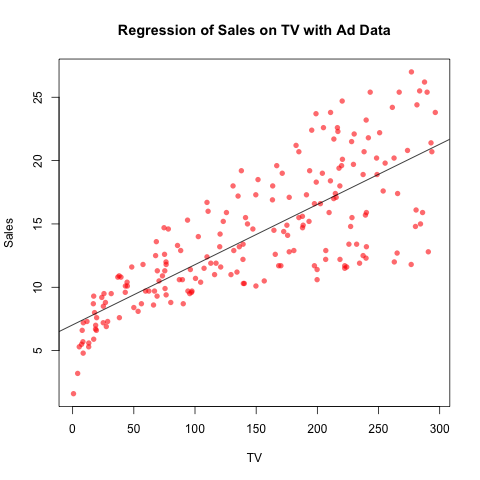
\includegraphics[width=250pt]{images/scatterplot-tv-sales.png}
\end{center}

Going deeper into this analysis, we focus our direction to the model and its quantitative properties. 

First we have the coefficients from this fitted regression given as below along with their std. errors and t-statistics.

\begin{table}[ht]
\centering
\begin{tabular}{rrrrr}
  \hline
 & Estimate & Std. Error & t value & Pr($>$$|$t$|$) \\ 
  \hline
(Intercept) & 7.0326 & 0.4578 & 15.36 & 0.0000 \\ 
  TV & 0.0475 & 0.0027 & 17.67 & 0.0000 \\ 
   \hline
\end{tabular}
\caption{Regression Output} 
\end{table}
From the intercept coefficient, we can see that if there was a \$0 ad budget then we would have 7.0325*1000 ~ 7032 units of sale. This represents the constant coefficient.

Moving on to the TV coefficient, we can understand that for every unit increase in TV budget the Sales would be impacted by +0.0475 units. Which means that if we increase the add budget by \$1000 then we would ideally see an increase in the sales by 47.5 units. This outlines the models ability to find a relationship between TV ads and actual Sales. Also, notice that the t-stat on the TV coefficient is 17.67 which indicates that this result is highly statistically significant.

From this, we know that allocation to the TV budget is actually efficient at increasing sales of the product. The model also helps in the prediction of the sales given a certain TV budget. This could help make future decisions about how much to allocate for marketing campaigns focused on TV.

Finally, to test whether this model is actually good we measure a few more variable. Please look at the table below.
\begin{table}[ht]
\centering
\begin{tabular}{rlr}
  \hline
 & Quantity & Value \\ 
  \hline
1 & Residual Standard Error & 3.26 \\ 
  2 & R2 & 0.61 \\ 
  3 & F-Statistic & 312.14 \\ 
   \hline
\end{tabular}
\caption{Measure of Fit Statistics} 
\end{table}
The first term "Residual Standard Error" measure the lack of fit of the model. This means that on average how much would the variance be from the given estimates. Here the value of 3.26 indicates that given the tv advertising the sales could be off by 3,2600 units on average. This error would be lower if the model had less variance which could make our estimate prediction better.

The second term $R^2$ is another measure of fit statistic. It describes the model in the form of proportions of variance in data explained by the model. Here 0.612 means that 61.2\% of the variance can be explained by this model.

Finally, the F-statistic is a measure of the statistical significance of the model. A value of 312.1 is high enough that we can say that the results are highly statistically significant.


\section{Conclusion}
Through this paper, we learn that TV ads play a significant role in increasing poduct sales. We also learn about the approximate quantitative difference tv ads made on sales for this given data. The results are statistically significant and 61.2\% of the variation can be explained by our linear model. This analysis can be helpful for anyone who is trying to understand the impact of tv ads dollars and how to allocate budgets accordingly. Finally, this is precisely why we see ads on tv. If it never increased sales then there would be no point of showing the advertisements. 



\end{document}
